%----------------------------------------------------------------------------------------
%	PACKAGES AND OTHER DOCUMENT CONFIGURATIONS
%----------------------------------------------------------------------------------------

\documentclass{article} % paper and 12pt font size

\newcommand\tab[1][1cm]{\hspace*{#1}}
\def\changemargin#1#2{\list{}{\rightmargin#2\leftmargin#1}\item[]}
\let\endchangemargin=\endlist 

\usepackage{amsmath,amsfonts,amsthm} % Math packages
\usepackage{fancyhdr}
\usepackage[catalan]{babel}
\usepackage[utf8]{inputenc}
\usepackage[T1]{fontenc}
\usepackage{xcolor}
\usepackage{textcomp}
\usepackage{graphicx}
\usepackage{float}
\usepackage{listings}
\usepackage{enumitem}
\usepackage{textgreek}
\usepackage{multirow,tabularx}
\graphicspath{ {img/} }
\setlength\parindent{0pt} % Removes all indentation from paragraphs - comment this line for an assignment with lots of text

\pagestyle{fancy}
\fancyhf{}
\lhead{PAC2 - Aprenentatge computacional}
\rhead{Jordi Alvaro Arqués}
\cfoot{\thepage}

\begin{document}


\section{Exercici 1}
\begin{enumerate}[label=\alph*]
	\item Construïu els models de classificació basats en el veí més proper emprant k=1 i k=3 a partir de l'arxiu "train.csv". És a dir, heu de construir els models 1NN i 3NN. Amb cada un d'aquests dos models heu de classificar els exemples de l'arxiu "test.csv"
\end{enumerate}
{\color{blue}
	Ens proporcionen un arxiu d'entrenament amb dades relacionat amb vins:\\

	{\fontfamily{pcr}\selectfont\small
	\begin{tabular}{l | r r r r r r r}
	 	& ALCOHOL & MALIC & MAGNESIUM & PHENOLS & FLAVANOIDS & COLOR & CLASS \\ \hline
		Train 1 & 13.16 & 2.36 & 101 & 2.8 & 3.24 & 5.68 & 0 \\
		Train 2 & 11.65 & 1.67 & 88 & 1.92 & 1.61 & 2.6 & 1 \\
		Train 3 & 12.25 & 1.73 & 80 & 1.65 & 2.03 & 3.4 & 1 \\
		Train 4 & 14.83 & 1.64 & 97 & 2.8 & 2.98 & 5.2 & 0 \\
		Train 5 & 13.05 & 1.73 & 92 & 2.72 & 3.27 & 7.2 & 0 \\
		Train 6 & 12.37 & 1.63 & 88 & 2.22 & 2.45 & 2.12 & 1 \\
		Train 7 & 13.87 & 1.9 & 107 & 2.95 & 2.97 & 4.5 & 0 \\
		Train 8 & 13.11 & 1.01 & 78 & 2.98 & 3.18 & 5.3 & 1 \\
	\end{tabular}
	} \\

	I el de test: \\

	{\fontfamily{pcr}\selectfont\small
	\begin{tabular}{l | r r r r r r r}
	 	& ALCOHOL & MALIC & MAGNESIUM & PHENOLS & FLAVANOIDS & COLOR & CLASS \\ \hline
		Test 1 & 14.22 & 3.99 & 128 & 3 & 3.04 & 5.1 & 0 \\
		Test 2 & 11.87 & 4.31 & 82 & 2.86 & 3.03 & 2.8 & 1 \\
	\end{tabular}
	} \\

	No hi ha valors absents, per tant, no els hem de tractar. Pel que fa als atributs, veiem que són numèrics i, tal i com es recomana al llibre de teoria de l'assignatura per al cas de valors numèrics, decidim aplicar estandardització per tal de normalitzar-los. A continuació, calcularem els promitjos i les desviacions estàndard.\\

	Per la característica "Alcohol" (ho marcarem amb el subíndex A), tenim el següent:

	\[mitjana_{A} = E(X_{A}) = \frac{1}{N}\sum\limits_{i=1}^N x_{Ai}\]
	\[mitjana_{A} = \frac{13.16 + 11.65 + 12.25 + 14.83 + 13.05 + 12.37 + 13.87 + 13.11}{8}\]
	\[mitjana_{A} = \frac{104.29}{8} = 13.04\]
	
	\[\sigma_{A} = \sqrt{\frac{1}{N}\sum\limits_{i=1}^N (x_{Ai}-E(X_A))^2}\]
	{\selectfont\tiny
	\begin{changemargin}{-2.5cm}{0.5cm}
		\[\sigma = \sqrt{\frac{(13.16-13.04)^2 + (11.65-13.04)^2 + (12.25-13.04)^2 + (14.83-13.04)^2 + (13.05-13.04)^2 + (12.37-13.04)^2 + (13.87-13.04)^2 + (13.11-13.04)^2}{8}} \]
	\end{changemargin}
	}
	\[\sigma_{A} = \sqrt{\frac{6.92}{8}}=0.93 \]

	Si ho repetim per a totes les altres acarcterístiques, obtenim la taula següent: \\ 

	{\fontfamily{pcr}\selectfont\small
	\begin{tabular}{c | r r r r r r}
		 & ALCOHOL & MALIC & MAGNESIUM & PHENOLS & FLAVANOIDS & COLOR \\ \hline
		 Mitjana & 13.04 & 1.71 & 91.38 & 2.50 & 2.72 & 4.50 \\
		\textsigma & 0.93 & 0.35 & 9.35 & 0.47 & 0.58 & 1.59 \\
	\end{tabular}
	}
	\\

	Ara normalitzem mitjançant el procediment d'estandarització totes les característiques de cada exemple. Ho fem de la següent manera:

	\[x_{Ai}' = \frac{x_{Ai} - E(X_{A})}{\sigma_{A}}\]
	\[x_{A1}' = \frac{13.16 - 13.04}{0.93} = 0.13\]


	i el resultat global del procés sobre les dades d'entrenament:\\

	{\fontfamily{pcr}\selectfont\small
	\begin{tabular}{l | r r r r r r r}
	 	& ALCOHOL & MALIC & MAGNESIUM & PHENOLS & FLAVANOIDS & COLOR & CLASS \\ \hline
		Train 1 & 0.13 & 1.88 & 1.03 & 0.62 & 0.90 & 0.74 & 0 \\
		Train 2 & -1.49 & -0.11 & -0.36 & -1.23 & -1.91 & -1.19 & 1 \\
		Train 3 & -0.85 & 0.06 & -1.22 & -1.80 & -1.18 & -0.69 & 1 \\
		Train 4 & 1.93 & -0.20 & 0.60 & 0.62 & 0.45 & 0.44 & 0 \\
		Train 5 & 0.01 & 0.06 & 0.07 & 0.45 & 0.95 & 1.70 & 0 \\
		Train 6 & -0.72 & -0.23 & -0.36 & -0.60 & -0.46 & -1.49 & 1 \\
		Train 7 & 0.90 & 0.55 & 1.67 & 0.94 & 0.44 & 0.00 & 0 \\
		Train 8 & 0.08 & -2.01 & -1.43 & 1.00 & 0.80 & 0.50 & 1 \\
	\end{tabular}
	} \\

	Per a les dades de test, també hi apliquem la mitjana i la desviació típica que hem trobat a partir de les dades d'entrenament (les dades de test no s'han utilitzat per a trobar aquests valors):\\

	{\fontfamily{pcr}\selectfont\small
	\begin{tabular}{l | r r r r r r r}
	 	& ALCOHOL & MALIC & MAGNESIUM & PHENOLS & FLAVANOIDS & COLOR & CLASS \\ \hline
		Test 1 & 1.27 & 6.58 & 3.92 & 1.04 & 0.56 & 0.38 & 0 \\
		Test 2 & -1.25 & 7.50 & -1.00 & 0.75 & 0.54 & -1.07 & 1 \\
	\end{tabular}
	} \\

	Per aplicar el kNN, calculem les distàncies euclidees de tots els exemples de test a tots els exemples de train: \\

	\[d_{X_iX_j} = \sqrt{\sum\limits_{k=1}^N (x_{ik}-x_{jk})^2}\]

	Per exemple, per a calcular la distància entre el test 1 i el train 1, fem el següent:
	
	\begin{changemargin}{-2.5cm}{0.5cm}
		\[d_{X_{Train_1}X_{Test_1}} = \sqrt{(0.13-1.27)^2 + (1.88-6.58)^2 + (1.03-3.92)^2 + (0.62-1.04)^2 + (0.90-0.56)^2 + (0.74-0.38)^2}\]
	\end{changemargin}

	\[d_{X_{Train_1}X_{Test_1}} = \sqrt{32.16}=5.67\]

	A continuació es mostra la taula amb els resultats finals per a tots els casos:

	{\fontfamily{pcr}\selectfont\small
	\begin{tabular}{r | r r}
		& Test 1 & Test 2 \\ \hline
		Train 1 & {\color{red} \textbf{5.67}} & {\color{red} \textbf{6.41}} \\
		Train 2 & 9.19 & 8.27 \\
		Train 3 & 9.25 & 8.07 \\
		Train 4 & {\color{olive} \textbf{7.58}} & 8.62 \\
		Train 5 & 7.82 & 8.12 \\
		Train 6 & 8.71 & {\color{olive} \textbf{7.96}} \\
		Train 7 & {\color{olive} \textbf{6.45}} & {\color{olive} \textbf{7.83}} \\
		Train 8 & 10.19 & 9.75 \\
	\end{tabular}
	} \\

	Per a 1NN, assignarem la classe 0 als dos exemples de test, ja que els valors de distàncies més petits (marcats en vermell) són amb el Train 1 que és de la classe 0, que correspon a una precisió del 50\% (recordem que el Test 1 pertany a la classe 0 i el Test 2 a la classe 1):
	\[presicio = \frac{1 + 0}{2} = 50\%\]

	
	Per al 3NN, busquem els següents valors més petits de distàncies i obtenim que els vots serien:

	\begin{itemize}
		\item Test 1: Train 1 (d = 5.67, vot = classe 0), Train 4 (d = 7.58, vot = classe 0) i Train 7 (d = 6.45, vot = classe 0). Predicció: 3 de 3 per a la classe 0, per tant, classe 0.
		\item Test 2: Train 1 (d = 6.41, vot = classe 0), Train 6 (d = 7.96, vot = classe 1) i Train 7 (d = 7.83, vot = classe 0). Predicció: 2 de 3 per a la classe 0, per tant, classe 0.
	\end{itemize}

	Això equival a una precisió del 50\%:
	\[presicio = \frac{1 + 0}{2} = 50\%\]

	Com a conlusió, podem dir que el mètode kNN per si sol no és capaç de classificar bé els exemples de test. Això és degut a que només valorant les distàncies de tots els atributs dels exemples de test amb els exemples d'entrenament no és suficient; hem de ponderar els atributs i saber quins són més rellevants. Això ho veurem a l'apartat d) d'aquest mateix exercici quan apliquem el kNN després d'haver-hi aplicat el PCA per tal de seleccionar els atributs més rellevants.
}
\begin{enumerate}[resume, label=\alph*]
	\item Construïu el model de classificació basat en k-means per a k=2 a partir de l'arxiu "train.csv". És a dir, heu de construir el model per a 2-means. Un cop tingueu el model heu de classificar els exemples de l'arxiu "test.csv".
\end{enumerate}
{\color{blue}
	En primer lloc, apliquem  el 2-means dues vegades sobre les dades estandaritzades: una per als 4 exemples de cadascuna de les classes. \\

	Comencem agafant com a centroides inicials els dos primers exemples (Train 1 i Train 4 per a la classe 0; Train 2 i Train 3 per a la classe 1): \\

	{\fontfamily{pcr}\selectfont\small
	\begin{tabular}{r r r r r r r}
	 	ALCOHOL & MALIC & MAGNESIUM & PHENOLS & FLAVANOIDS & COLOR & CLASS \\ \hline
		0.13 & 1.88 & 1.03 & 0.62 & 0.90 & 0.74 & 0 \\
		1.93 & -0.20 & 0.60 & 0.62 & 0.45 & 0.44 & 0 \\
		-1.49 & -0.11 & -0.36 & -1.23 & -1.91 & -1.19 & 1 \\
		-0.85 & 0.06 & -1.22 & -1.80 & -1.18 & -0.69 & 1 \\
	\end{tabular}
	} \\

	Ara, es calculen les distàncies euclídees per als exemples de cada grup respecte els centroides escollits. Ja hem vist com es calculava la distància euclídea a l'exercici anterior, per tant, només mostrarem la taula de distàncies després de fer la primera iteració per al grup de la classe 1 (només apliquen els exemples de training 2, 3, 6 i 8): \\

	{\fontfamily{pcr}\selectfont\small
	\begin{tabular}{r | r r}
		& Centroide 1 & Centroide 2 \\ \hline
		Train 2 & \textbf{0.00} & 1.51 \\
		Train 3 & 1.51 & \textbf{0.00} \\
		Train 6 & \textbf{1.79} & 1.86 \\
		Train 8 & 4.73 & \textbf{4.29} \\
	\end{tabular}
	} \\

	Llavors, després de la primera iteració, calculem els nous centroides per a la classe 1. Primer, seleccionem els exemples de training més propers a cada centroide. Per tant, tenim que:\\

	\begin{itemize}
		\item[] Centroide 1: \{Train 2, Train 6\}
		\item[] Centroide 2: \{Train 3, Train 8\}
	\end{itemize}

	Ara, calculem els valors de les característiques dels nous centroides a partir dels exemples que hi pertanyen. Això s'aconsegueix fent la mitjana aritmètica. Per exemple, per a la característica "Alcohol" del centroide 1 (de la classe 1), tenim que el nou valor serà: \\

	\[c'_A = \frac{x_{A2} + x_{A6}}{2} = \frac{-1.49 + (-0.72)}{2}=-1.10\]

	Llavors, els nous centroides seran: \\

	{\fontfamily{pcr}\selectfont\small
	\begin{tabular}{r r r r r r r}
	 	ALCOHOL & MALIC & MAGNESIUM & PHENOLS & FLAVANOIDS & COLOR & CLASS \\ \hline
		-1.10 & -0.17 & -0.36 & -0.92 & -1.18 & -1.34 & 1 \\
		-0.38 & -0.98 & -1.32 & -0.40 & -0.19 & -0.09 & 1 \\
	\end{tabular}
	} \\

	A partir d'aquí, es tornaria a calcular les distàncies euclídees i els nous centroides. Aquest procés es repetiria fins que arribem a un cert nombre màxim d'iteracions o bé no hi ha cap modificació a les particions (dintre del grup escollit, en aquest cas el grup de classe 1). \\

	El mateix procediment es repeteix per a la classe 0 (no mostrem el procés). \\

	Finalment, obtenim els 4 centroides resultants:\\

	{\fontfamily{pcr}\selectfont\small
	\begin{tabular}{r r r r r r r}
	 	ALCOHOL & MALIC & MAGNESIUM & PHENOLS & FLAVANOIDS & COLOR & CLASS \\ \hline
		0.07 & 0.97 & 0.55 & 0.54 & 0.93 & 1.22 & 0 \\
		1.41 & 0.18 & 1.14 & 0.78 & 0.45 & 0.22 & 0 \\
		-1.02 & -0.09 & -0.65 & -1.21 & -1.18 & -1.13 & 1 \\
		0.08 & -2.01 & -1.43 & 1.00 & 0.80 & 0.50 & 1 \\
	\end{tabular}
	} \\

	Apliquem 1NN agafant com a training els quatre centroides obtinguts en el pas anterior i com a test el conjunt de test. El tractarem com hem fet a l'exercici anterior. Obtenim les distàncies següents:\\

	{\fontfamily{pcr}\selectfont\small
	\begin{tabular}{r | r r}
	 	& Test 1 & Test 2 \\ \hline
		Centroide 1 & {\color{red} \textbf{6.73}} & {\color{red} \textbf{7.23}} \\
		Centroide 2 & 6.99 & 8.18 \\
		Centroide 3 & 9.00 & 8.04 \\
		Centroide 4 & 10.19 & 9.75 \\
	\end{tabular}
	} \\

	Per a 1NN, assignarem la classe 0 a ambdós exemples, ja que els més petits (marcats en vermell) són d’aquestes classes, que correspon a una precisió del 50\% (recordem que l'exemple 1 pertany a la classe 0 i el 2 a la classe 1): \\
	\[presicio = \frac{1 + 0}{2} = 50\%\]

	En aquest cas, podem veure que l'aplicació de k-means supervisat (k=2) + 1NN no acaba d'aportar-nos una millora substancial. Els valors del Test 2 segueixen estant més allunyats dels centroides que classifiquen la classe 1. En comparació amb el kNN aplicat directament a l'apartat anterior, el centroide 3 (classe 1) s'ha apropat més al Test 2, però aquest encara segueix més proper al centroide 1 (classe 0). \\
}

\begin{enumerate}[resume, label=\alph*]
	\item Construïu un arbre de decisió a partir de l'arxiu "train.csv". Un cop tingueu l'arbre, classifiqueu amb ell els exemples de l'arxiu "test.csv". 
\end{enumerate}
{\color{blue}
	Per a construir arbres de decisió no cal normalitzar, donat que no treballarem amb distàncies. \\

	Tots els atributs són numèrics. Utilitzarem els punts de tall per tractar-los. Els punts de tall es calculen ordenant tots els valors d'un atribut (eliminant les repeticions si n’hi ha) i calculant la mitjana aritmètica de cada dos valors consecutius. \\

	Per exemple, el primer valor llindar de l'atribut "Alcohol", s'han ordenat els valors, eliminat els repetits i agafat els dos primers valors. Llavors obtenim: \\
	\[llindar_1 = \frac{11.65 + 12.25}{2} = 11.95\]

	A continuació es mostra les taules finals dels valors ordenats sense repeticions i els seus punts de tall per a tots els atributs. L'últim valor de cada atribut no té un llindar assignat ja que és el valor més gran i, per tant, no hi ha un valor superior amb el que promitjar. \\


	{\fontfamily{pcr}\selectfont\small
	\begin{tabular}{r | r}
	 	\multicolumn{2}{c}{ALCOHOL}  \\ \hline
	 	Valor & Llindar \\ \hline
		11.65 & 11.95 \\
		12.25 & 12.31 \\
		12.37 & 12.71 \\
		13.05 & 13.08 \\
		13.11 & 13.135 \\
		13.16 & 13.515 \\
		13.87 & 14.35 \\
		14.83 &  \\
	\end{tabular}
	} \\

	{\fontfamily{pcr}\selectfont\small
	\begin{tabular}{r | r}
	 	\multicolumn{2}{c}{MALIC}  \\ \hline
	 	Valor & Llindar \\ \hline
		1.01 & 1.32 \\
		1.63 & 1.635 \\
		1.64 & 1.655 \\
		1.67 & 1.7 \\
		1.73 & 1.815 \\
		1.9 & 2.13 \\
		2.36 &  \\
	\end{tabular}
	} \\

	{\fontfamily{pcr}\selectfont\small
	\begin{tabular}{r | r}
	 	\multicolumn{2}{c}{MAGNESIUM}  \\ \hline
	 	Valor & Llindar \\ \hline
		78 & 79 \\
		80 & 84 \\
		88 & 90 \\
		92 & 94.5 \\
		97 & 99 \\
		101 & 104 \\
		107 &  \\
	\end{tabular}
	} \\

	{\fontfamily{pcr}\selectfont\small
	\begin{tabular}{r | r}
	 	\multicolumn{2}{c}{PHENOLS} \\ \hline
	 	Valor & Llindar \\ \hline
		1.65 & 1.785 \\
		1.92 & 2.07 \\
		2.22 & 2.47 \\
		2.72 & 2.76 \\
		2.8 & 2.875 \\
		2.95 & 2.965 \\
		2.98 &  \\
	\end{tabular}
	} \\

	{\fontfamily{pcr}\selectfont\small
	\begin{tabular}{r | r}
	 	\multicolumn{2}{c}{FLAVANOIDS} \\ \hline
	 	Valor & Llindar \\ \hline
		1.61 & 1.82 \\
		2.03 & 2.24 \\
		2.45 & 2.71 \\
		2.97 & 2.975 \\
		2.98 & 3.08 \\
		3.18 & 3.21 \\
		3.24 & 3.255 \\
		3.27 &  \\
	\end{tabular}
	} \\
	
	{\fontfamily{pcr}\selectfont\small
	\begin{tabular}{r | r}
	 	\multicolumn{2}{c}{COLOR} \\ \hline
	 	Valor & Llindar \\ \hline
		2.12 & 2.36 \\
		2.6 & 3 \\
		3.4 & 3.95 \\
		4.5 & 4.85 \\
		5.2 & 5.25 \\
		5.3 & 5.49 \\
		5.68 & 6.44 \\
		7.2 &  \\
	\end{tabular}
	} \\

	Anem ara a veure com de bo és cada llindar. El que farem per a cada llindar és dividir els exemples en dos grups: aquells que són menors que el llindar i aquells que són majors. \\

	Seguim treballant amb l'atribut "Alcohol". Comencem pel llindar 11.95 i dividim els exemples en dos grups. Si observem la taula inicial de les dades d'entrenament podem veure que "Train 2" està per davall de 11.95 mentre que la resta estan per damunt. Ara se'ns presenten dues opcions:

	\begin{itemize}
		\item Suposar que els exemples amb valor inferior a 11.95 pertanyen a la classe 1 i els que tenen un valor superior a 11.95 pertanyen a la classe 0. Així, tindríem un exemple ben classificat per davall del llindar (Train 2) i quatre de ben classificats per damunt (Train 1, Train 4, Train 5 i Train 7). En total, cinc exemples ben classificats.
		\item Suposar que els exemples amb valor inferior a 11.95 pertanyen a la classe 0 i els que tenen un valor superior a 11.95 pertanyen a la classe 1. En aquest cas, l’exemple que està per davall del llindar estaria mal classificat, i per damunt del llindar en tindríem tres (Train 3, Train 6 i Train 8) de ben classificats. En total, tres exemples ben classificats.
	\end{itemize}

	La bondat de la primera suposició seria de cinc exemples correctes d’un total de vuit. És a dir, 5/8=62.5\%. La bondat de la segona suposició seria de tres exemples correctes d’un total de vuit. És a dir, 3/8=37.5\%. Ja que la decisió de com interpretar el llindar és arbitrària, ens quedem amb la millor possibilitat: la primera. \\

	Si continuem amb la resta de llindars, obtenim els resultats mostrats a les següents taules per a tots els atributs. La taula ens mostra la bondat i el criteri a seguir per aconseguir aquesta bondat. \\

	{\fontfamily{pcr}\selectfont\small
	\begin{tabular}{r | l | r}
	 	\multicolumn{3}{c}{ALCOHOL}  \\ \hline
	 	Llindar & Bondat & Criteri \\ \hline
		11.95  & (1+4)/8 = 62.5\% & menor és classe 1 \\
		12.31  & (2+4)/8 = 75\% & menor és classe 1 \\
		12.71  & \textbf{(3+4)/8 = 87.5\%} & menor és classe 1 \\
		13.08  & (3+3)/8 = 75\% & menor és classe 1 \\
		13.135 & \textbf{(4+3)/8 = 87.5\%} & menor és classe 1 \\
		13.515 & (4+2)/8 = 75\% & menor és classe 1 \\
		14.35  & (4+1)/8 = 62.5\% & menor és classe 1 \\
	\end{tabular}
	} \\

	{\fontfamily{pcr}\selectfont\small
	\begin{tabular}{r | l | r}
	 	\multicolumn{3}{c}{MALIC}  \\ \hline
	 	Llindar & Bondat & Criteri \\ \hline
		1.32  & (1+4)/8 = 62.5\% & menor és classe 1 \\
		1.635 & \textbf{(2+4)/8 = 75\%} & menor és classe 1 \\
		1.655 & (2+3)/8 = 62.5\% & menor és classe 1 \\
		1.7   & \textbf{(3+3)/8 = 75\%} & menor és classe 1 \\
		1.815 & \textbf{(4+2)/8 = 75\%} & menor és classe 1 \\
		2.13  & (4+1)/8 = 62.5\% & menor és classe 1 \\
	\end{tabular}
	} \\

	{\fontfamily{pcr}\selectfont\small
	\begin{tabular}{r | l | r}
	 	\multicolumn{3}{c}{MAGNESIUM}  \\ \hline
	 	Llindar & Bondat & Criteri \\ \hline
		79   & (1+4)/8 = 62.5\% & menor és classe 1 \\
		84   & (2+4)/8 = 75\% & menor és classe 1 \\
		90   & \textbf{(4+4)/8 = 100\%} & menor és classe 1 \\
		94.5 & (4+3)/8 = 87.5\% & menor és classe 1 \\
		99   & (4+2)/8 = 75\% & menor és classe 1 \\
		104  & (4+1)/8 = 62.5\% & menor és classe 1 \\
	\end{tabular}
	} \\

	{\fontfamily{pcr}\selectfont\small
	\begin{tabular}{r | l | r}
	 	\multicolumn{3}{c}{PHENOLS} \\ \hline
	 	Llindar & Bondat & Criteri \\ \hline
		1.785 & (1+4)/8 = 62.5\% & menor és classe 1 \\
		2.07  & (2+4)/8 = 75\% & menor és classe 1 \\
		2.47  & \textbf{(3+4)/8 = 87.5\%} & menor és classe 1 \\
		2.76  & (3+3)/8 = 75\% & menor és classe 1 \\
		2.875 & (3+1)/8 = 50\% & menor és classe 1 \\
		2.965 & (4+1)/8 = 62.5\% & menor és classe 0 \\
	\end{tabular}
	} \\

	{\fontfamily{pcr}\selectfont\small
	\begin{tabular}{r | l | r}
	 	\multicolumn{3}{c}{FLAVANOIDS} \\ \hline
	 	Llindar & Bondat & Criteri \\ \hline
		1.82  & (1+4)/8 = 62.5\% & menor és classe 1 \\
		2.24  & (2+4)/8 = 75\% & menor és classe 1 \\
		2.71  & \textbf{(3+4)/8 = 87.5\%} & menor és classe 1 \\
		2.975 & (3+3)/8 = 75\% & menor és classe 1 \\
		3.08  & (3+2)/8 = 62.5\% & menor és classe 1 \\
		3.21  & (4+2)/8 = 75\% & menor és classe 1 \\
		3.255 & (4+1)/8 = 62.5\% & menor és classe 1 \\
	\end{tabular}
	} \\
	
	{\fontfamily{pcr}\selectfont\small
	\begin{tabular}{r | l | r}
	 	\multicolumn{3}{c}{COLOR} \\ \hline
	 	Llindar & Bondat & Criteri \\ \hline
		2.36 & (1+4)/8 = 62.5\% & menor és classe 1 \\
		3    & (2+4)/8 = 75\% & menor és classe 1 \\
		3.95 & \textbf{(3+4)/8 = 87.5\%} & menor és classe 1 \\
		4.85 & (3+3)/8 = 75\% & menor és classe 1 \\
		5.25 & (3+2)/8 = 62.5\% & menor és classe 1 \\
		5.49 & (4+2)/8 = 75\% & menor és classe 1 \\
		6.44 & (4+1)/8 = 62.5\% & menor és classe 1 \\
	\end{tabular}
	} \\

	Cal notar que a l'últim llindar dels phenols hem escollit el criteri "menor és classe 0", ja que amb el criteri "menor és classe 1"\ aconseguiem una bondat menor al 50\%, en concret del 37.5\%. \\

	També, cal mencionar que hem marcat els millors llindars per a cada atribut en negreta, que són els que ens quedarem. En cas d'empat, n'escollim un aleatòriament. \\

	De totes les bondats que hem calculat, el millor cas es dóna amb l’atribut "Magnesium"\ i el llindar 90, amb el que aconseguim un 100\% de bondat. Tenim particionat correctament el conjunt d’exemples. Sinó haguéssim aconseguit un 100\% de bondat a la primera iteració, hauríem d'haver hagut de repetir el procés de cerca de llindars i bondats per a cada una de les branques que no estan completament classificades. \\

	Així, hem enllestit la construcció de l'arbre, que quedaria:

	\begin{figure}[H]
		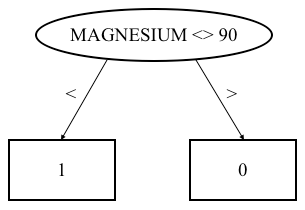
\includegraphics[width=6cm]{magnesiumtree}
		\centering
		\color{blue}
		\caption{arbre de decisió creat a partir de l'arxiu train.csv.}\label{visina8}
	\end{figure}

	Si apliquem el conjunt de test a l'arbre que acabem de crear, veiem que classifica correctament els dos exemples. Les prediccions són classe 0 i classe 1 respectivament:

	\begin{itemize}
		\item Test 1 té un valor de 128 per a "Magnesium"\ i, per tant, el classifica com a classe 0.
		\item Test 2 té un valor de 82 per a "Magnesium"\ i, per tant, el classifica com a classe 1.
	\end{itemize}

	La precisió serà:
	\[presicio = \frac{1 + 1}{2} = 100\%\]

	Com a conclusió, cal dir que, en aquest cas, la tècnica de l'arbre de decisió ha estat molt precís i ha sabut trobar la característica principal que ens permet classificar correctament els exemples de test. De totes formes, en aquest exercici estem tractant amb quantitats de dades molt reduïdes i és complicat d'extrapolar aquest resultat a conjunts de dades més grans i realistes. \\
	 
}

\begin{enumerate}[resume, label=\alph*]
	\item Apliqueu PCA per a reduir la dimensionalitat dels conjunts anteriors conservant el 95\% de la variància. Utilitzeu ara 1NN i 3NN sobre els conjunts reduïts de la mateixa forma que en el primer apartat. Compareu els resultats. Indiqueu clarament les diferències en aplicar PCA sobre el conjunt d'entrenament i sobre el de test.
\end{enumerate}

{\color{blue} \leftmargin=4in
	Apliquem el PCA sobre el conjunt de l'arxiu d'entrenament. Primer obtenim els valors propis: \\

	{\fontfamily{pcr}\selectfont\small
	\begin{tabular}{r r r r r r}
		3.58 & 1.49 & 0.56 & 0.24 & 0.11 & 0.02 \\
	\end{tabular}
	} \\

	I els vectors propis: \\

	{\fontfamily{pcr}\selectfont\small
	\begin{tabular}{r r r r r r}
		-0.45 &  -0.05 &  -0.55 &  0.66 &  -0.19 &  0.14 \\
		-0.13 &  0.75 &  0.36 &  0.09 &  -0.36 &  0.38 \\
		-0.35 &  0.56 &  -0.3 &  -0.21 &  0.46 &  -0.47 \\
		-0.49 &  -0.19 &  -0.16 &  -0.57 &  0.11 &  0.6 \\
		-0.49 &  -0.2 &  0.22 &  -0.23 &  -0.6 &  -0.5 \\
		-0.43 &  -0.19 &  0.63 &  0.36 &  0.5 &  0.01 \\
	\end{tabular}
	} \\

	A continuació, Obtenim els percentatges de variàncies dels components principals: \\

	{\fontfamily{pcr}\selectfont\small
	\begin{tabular}{r r r r r r}
		0.60 & 0.25 & 0.09 & 0.04 & 0.02 & 0.00 \\
	\end{tabular}
	} \\

	Si les acumulem: \\

	{\fontfamily{pcr}\selectfont\small
	\begin{tabular}{r r r r r r}
		0.60 & 0.84 & 0.94 & 0.98 & 1.00 & 1.00 \\
	\end{tabular}
	} \\

	Per tant, veiem que només necessitem 4 components principals per tal de mantenir el 95\% de la variància de les dades inicials. Si apliquem la conversió, obtenim la següent taula (hem reduït 2 dimensions): \\

	{\fontfamily{pcr}\selectfont\small
	\begin{tabular}{r | r r r r}
		Train 1 & -1.73 & 1.55 & 0.87 & -0.25 \\
		Train 2 & 2.85 & 0.63 & -0.1 & -0.21 \\
		Train 3 & 2.55 & 0.12 & 0.44 & 0.75 \\
		Train 4 & -1.76 & -0.21 & -1.03 & 0.83 \\
		Train 5 & -1.45 & -0.52 & 1.21 & 0.14 \\
		Train 6 & 1.64 & 0.15 & -0.53 & -0.51 \\
		Train 7 & -1.73 & 1.04 & -0.85 & -0.34 \\
		Train 8 & -0.37 & -2.77 & -0.01 & -0.4 \\
	\end{tabular}
	} \\

	No obstant, hem perdut el significat de cadascuna de les característiques. N’hi ha quatre de noves que són una combinació lineal de les inicials, en base als vectors i valors propis que s’han obtingut mitjançant el PCA. \\

	Cal comentar que l'aplicació del PCA per a obtenir els valors i vectors propis s'ha de fer únicament sobre les dades d'entrenament. Un cop trobats aquests components, podem aplicar-los sobre les dades de test per a obtenir les seves projeccions. No obstant, les dades de test no poden formar mai part de les dades inicials per a calcular aquests valors i vectors propis. \\

	Ara, utilitzarem els valors i vectors propis obtinguts prèviament amb les dades d'entrenament per tal de calcular la versió reduïda de les dades de test: \\

	{\fontfamily{pcr}\selectfont\small
	\begin{tabular}{r | r r r r}
		Test 1 & -2.07 & -0.82 & -0.52 & -0.08 \\
		Test 2 & 2.07 & 0.82 & 0.52 & 0.08 \\
	\end{tabular}
	} \\

	Un cop obtingudes les dades projectades, fem el mateix que al primer apartat, per tal de calcular la matriu de distàncies i obtenim: \\

	{\fontfamily{pcr}\selectfont\small
	\begin{tabular}{r | r r}
		 & Test 1 & Test 2 \\\hline
		Train 1 & 2.78 & 3.90 \\
		Train 2 & 5.15 & {\color{red} \textbf{1.05}} \\
		Train 3 & 4.88 & {\color{olive} \textbf{1.09}} \\
		Train 4 & {\color{red} \textbf{1.25}} & 4.33 \\
		Train 5 & {\color{olive} \textbf{1.87}} & 3.83 \\
		Train 6 & 3.86 & {\color{olive} \textbf{1.44}} \\
		Train 7 & {\color{olive} \textbf{1.94}} & 4.06 \\
		Train 8 & 2.66 & 4.40 \\
	\end{tabular}
	} \\

	Per a 1NN, busquem els valors més petits de distàncies (marcats en vermell) i obtenim que els vots serien:

	\begin{itemize}
		\item Test 1: Train 4 (d = 1.25, vot = classe 0). Predicció: classe 0.
		\item Test 2: Train 2 (d = 1.05, vot = classe 1). Predicció: classe 1.
	\end{itemize}

	Això equival a una precisió del 100\%:
	\[presicio = \frac{1 + 1}{2} = 100\%\]

	
	Per al 3NN, busquem els següents valors més petits de distàncies i obtenim que els vots serien:

	\begin{itemize}
		\item Test 1: Train 4 (d = 1.25, vot = classe 0), Train 5 (d = 1.87, vot = classe 0) i Train 7 (d = 1.94, vot = classe 0). Predicció: 3 de 3 per a la classe 0, per tant, classe 0.
		\item Test 2: Train 2 (d = 1.05, vot = classe 1), Train 3 (d = 1.09, vot = classe 1) i Train 6 (d = 1.44, vot = classe 1). Predicció: 3 de 3 per a la classe 1, per tant, classe 1.
	\end{itemize}

	Això equival a una precisió del 100\%:
	\[presicio = \frac{1 + 1}{2} = 100\%\]

	Si comparem les precisions obtingudes aplicant el PCA + kNN respecte de l'apartat a) d'aquest exercici on només s'ha aplicat kNN, podem veure una gran millora ja que amb kNN sol només hem aconseguit classificar bé un dels dos exemples de test, mentres que amb PCA + kNN ha classificat correctament els dos. \\

	També podem observar que les distàncies mínimes entre els exemples de test i entrenament de la matriu de distàncies han variat amb l'aplicació de PCA. Això és degut a que PCA ens selecciona els atributs més representatius i que més informació ens aporten sobre les dades. De fet, amb l'aplicació del PCA, el 3NN ha encertat plenament (distàncies mínimes de la classe correcta: 3 de 3) la classe dels dos exemples de test, mentres que sense l'aplicació del PCA no havia estat així. \\
}


\section{Exercici 2}
L'objectiu d'aquest exercici és la construcció d'un model amb un conjunt de dades realista. Per a realitzar aquest exercici teniu a la vostra disposició la biblioteca sklearn per a Python: \\

http://scikit-learn.org \\

L'arxiu adjunt "wine.csv"\ conté més de 100 exemples de vins en un format fàcilment llegible des de Python. Se us demana l'estudi de cara a construir un classificador. En particular, heu de:
\begin{itemize}
	\item Provar els algorismes de validació creuada (\textit{cross-validation}). És a dir, no heu d'utilitzar un sol conjunt d'entrenament i un sol conjunt de test. La biblioteca sklearn proporciona iteradors específicament dissenyats per a aquesta tasca, com ara \textit{KFold}, \textit{RepeatedKFold}, \textit{GroupKFold}, \textit{StratifiedKFold}. Llegiu-ne la documentació i concentrau-vos en un d'ells.
	\item Provar almenys els algorismes: KNN, algun tipus de SVM, xarxes neuronals (perceptró multicapa) i algun altre classificador de la vostra elecció.
\end{itemize}
Comenteu els resultats obtinguts i justifiqueu tot el que feu.
\\

{\color{blue}
	En aquest exercici estudiarem com es comporten diferents algorismes classificadors. Partim de l'arxiu "wine.csv"\ i per tal de poder realitzar l'estudi utilitzarem un dels algorismes disponibles a la llibreria sklearn de validació creuada, en concret el RepeatedKFold. \\

	L'algorisme KFold de validació creuada divideix les dades en k subconjunts (o n\_splits) d'una mateixa grandària (sempre que es pugui). Les mostres de cada subconjunt poden ser escollides aleatòriament o no (consecutivament). \\

	Llavors, cada subconjunt s'utilitza una vegada per a la predicció, mentre que els k-1 restants formen el subconjunt d'aprenentatge per a aquella iteració. En total es realitzen k iteracions. \\

	L'algorisme RepeatedKFold es basa en els mateixos conceptes que el KFold, però afegeix la possibilitat que tot el procés es pugui repetir n vegades (o n\_repeats). \\

	Nosaltres hem decidit aplicar el RepeatedKFold amb els següents paràmetres:
	{\fontfamily{pcr}\selectfont\small
	\begin{itemize}
		\item n\_splits = 10
		\item n\_repeats = 10
	\end{itemize}
	}

	En concret, el codi que inicialitza el KFold seria: \\

	{\fontfamily{pcr}\selectfont\small
		rkf = RepeatedKFold(n\_splits=10, n\_repeats=10)
	} \\

	Per tant, sabent que l'arxiu "wines.csv"\ conté un total de 122 mostres, després d'aplicar el RepeatedKFold, obtindrem una matriu de confusió amb una població total de 1220 mostres (122 mostres * 10 repeticions). \\

	A continuació es mostren els resultats per als diferents algoritmes de classificació utilitzats. Els resultats mostrats fan referència a les estadístiques dels temps d'aprenentatge i predicció i a la matriu de confusió. \\

	Com a referència, la següent taula mostra un resum dels valors mostrats en relació a la matriu de confusió:

	\begin{figure}[H]
		\begin{changemargin}{-4.5cm}{0.5cm}
			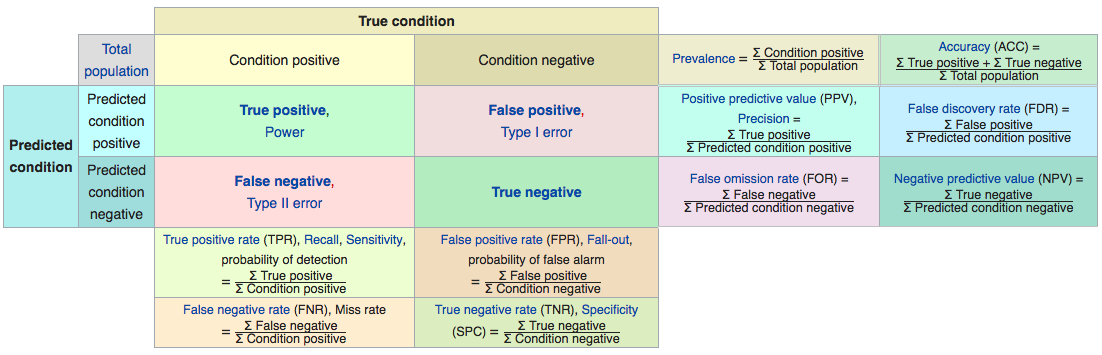
\includegraphics[width=21cm]{confusionmatrix}
			\centering
			\color{blue}
			\caption{Matriu de confusió ampliada.}\label{visina8}
		\end{changemargin}
	\end{figure}


	Els algorismes de classificació de la llibreria scikit que s'han utilitzat són:
	\begin{itemize}
		\item {
			KNeighborsClassifier amb n\_neighbors = 1. És un classificador kNN (k Nearest Neighbors) amb k = 1. \\
			{\fontfamily{pcr}\selectfont\small
				clf = KNeighborsClassifier(n\_neighbors=1)
			}
		}
		\item {
			KNeighborsClassifier amb n\_neighbors = 3. És un classificador kNN (k Nearest Neighbors) amb k = 3. \\
			{\fontfamily{pcr}\selectfont\small
				clf = KNeighborsClassifier(n\_neighbors=3)
			}
		}
		\item {
			SVC. És un classificador de la família dels SVM (Support Vector Machines). \\
			{\fontfamily{pcr}\selectfont\small
				clf = SVC()
			}
		}
		\item {
			MLPClassifier. És un classificador de la família de les xarxes neuronals i implementa un algorisme perceptró multicapa (MLP). Alguns dels paràmetres escollits per a aquest classificador són:
			{
			\begin{itemize}
				\item Rectificador lineal: \[f(x) = max(0, x)\]
				\item Solver: un optimitzador de la família dels mètodes quasi-Newton.
				\item Alpha: paràmetre de regularització L2
				\item Hidden layers: Hem definit 5 neurones per a la primera capa i 2 per a la segona.
			\end{itemize}
			}
			{\fontfamily{pcr}\selectfont\small
				clf = MLPClassifier(solver='lbfgs', alpha=1e-5, hidden\_layer\_sizes=(5, 2), random\_state=1)
			}
		}
		\item {
			SGDClassifier. És un classificador de la família dels SGD (Stochastic Gracient Descent).  Alguns dels paràmetres escollits per a aquest classificador són:
			{
			\begin{itemize}
				\item Funció de pèrdua: SVM lineal
				\item Penalty: paràmetre de regularització L2
			\end{itemize}
			}
			{\fontfamily{pcr}\selectfont\small
				clf = SGDClassifier(loss='hinge', penalty='l2')
			}
		}
	\end{itemize}

	A continuació, es pot observar una taula comparativa de tots els resultats i mètriques dels diferents classificadors: \\

	\begin{changemargin}{-2.5cm}{0.5cm}
	{\fontfamily{pcr}\selectfont\small
	\begin{tabular}{l | r r r r r}
		& 1NN & 3NN & SVC & MLP & SGD \\ \hline
		Average Train times & 0.3603 ms & 0.3449 ms & 0.5576 ms & 4.5121 ms & 0.4559 ms \\
		Standard deviation Train times & 0.2064 ms & 0.0822 ms & 0.1902 ms & 0.5129 ms & 0.4353 ms \\ \hline
		Average Predict times & 0.4227 ms & 0.4131 ms & 0.0976 ms & 0.1131 ms & 0.0614 ms \\
		Standard deviation Predict times & 0.0593 ms & 0.0563 ms & 0.0306 ms & 0.0138 ms & 0.0631 ms \\ \hline
		True positive & 621 & 622 & 670 & 654 & 649 \\
		False positive & 0 & 0 & 5 & 4 & 21 \\
		False negative & 49 & 48 & 0 & 16 & 21 \\
		True negative & 550 & 550 & 545 & 546 & 529 \\ \hline
		Prevalence & 54.92\% & 54.92\% & 54.92\% & 54.92\% & 54.92\% \\
		Accuracy & 95.98\% & 96.07\% & 99.59\% & 98.36\% & 96.56\% \\ \hline
		Precision & 100.0\% & 100.0\% & 99.26\% & 99.39\% & 96.87\% \\
		False discovery rate & 0.0\% & 0.0\% & 0.74\% & 0.61\% & 3.13\% \\
		False omission rate & 8.18\% & 8.03\% & 0.0\% & 2.85\% & 3.82\% \\
		Negative predictive value & 91.82\% & 91.97\% & 100.0\% & 97.15\% & 96.18\% \\ \hline
		Recall & 92.69\% & 92.84\% & 100.0\% & 97.61\% & 96.87\% \\
		Fall-out & 0.0\% & 0.0\% & 0.91\% & 0.73\% & 3.82\% \\
		False negative rate & 7.31\% & 7.16\% & 0.0\% & 2.39\% & 3.13\% \\
		Specificity & 100.0\% & 100.0\% & 99.09\% & 99.27\% & 96.18\% \\ \hline
		Classificacions correctes & 1171 & 1172 & 1215 & 1200 & 1178 \\
		Classificacions incorrectes & 49 & 48 & 5 & 20 & 42 \\
	\end{tabular}
	}
	\end{changemargin}
	
	I si analitzem per separat les matrius bàsiques de confusió tenim que: \\

	{\fontfamily{pcr}\selectfont\small
	\begin{tabular}{l | r r | r}
		1NN & 621 & 0 & a = 1 \\
		& 49 & 550 & b = 0 \\ \hline
		3NN & 622 & 0 & a = 1 \\
		& 48 & 550 & b = 0 \\ \hline
		SVC & 670 & 5 & a = 1 \\
		& 0 & 545 & b = 0 \\ \hline
		MLP & 654 & 4 & a = 1 \\
		& 16 & 546 & b = 0 \\ \hline
		SGD & 649 & 21 & a = 1 \\
		& 21 & 529 & b = 0 \\
	\end{tabular}
	} \\

	És important valorar que tots els algorismes tenen una accuracy molt elevada (per sobre del 95\%), però cal destacar el SVC que amb un 99.59\% és el que millors resultats dóna en aquest sentit. Molt seguit trobem el MLP i, pràcticament empatats en última posició, el SGD, 3NN i 1NN. L'accuracy és un paràmetre dirèctament relacionat amb el nombre de classificacions directes i, tal i com es pot observar a la taula, el SVC n'ha obtingut el màxim valor amb 1215 (5 d'incorrectes).\\

	De totes maneres, pel que fa a la precisió els 1NN i 3NN han obtingut un 100\% sent el SGD el pitjor amb un 96.87\%. Això ens indica que té una tendència més marcada a predir la classe 1 i, en aquests casos, s'equivoca més sovint que els altres algorismes. \\

	També, cal remarcar el valor del Negative predictive value, a on el SVC torna a despuntar amb un 100\% d'encerts. Això ens indica que aquest algoritme detecta amb molta fiabilitat la classe 0. En altres paraules, quan prediu que un vi és de tipus 0, segurament ho serà. Per contra, els algorismes 1NN i 3NN tenen problemes a l'hora de predir la classe 0, això també és pot observar mirant el valor dels falsos negatius (49 i 48 respectivament, mentres que el SVC n'ha obtingut 0). Una altra forma de d'arribar a aquestes conclusions seria mirar el valor False omission rate per a cadascun d'ells.\\

	Si ara mirem els resultats obtinguts pel valor Recall (o Sensitivity), tornem a confirmar els bons resultats de l'algoritme SVC. En aquest senttit, ha obtingut un 100\% superant tots els altres algorismes (1NN amb 92.69\%, 3NN amb 92.84\%, MLP amb 97.61\% i SGD amb 96.87\%). Això ens indica que de tots els vins que eren de classe 1, n'ha predit correctament el 100\%. \\

	Per tant, veiem que l'únic punt dèbil de l'algorisme SVC amb aquest conjunt de dades són els falsos positius. \\

	Pel que fa a l'anàlisi dels temps de construcció del model dels diferents algorismes, podem observar que la construcció del model MLP (xarxes neuronals) és molt costosa (entre 8 i 13 vegades més lenta de mitjana). D'altra banda, té una desviació típica bastant similar als altres algorismes, tret del 3NN que és menor. Comparant la mitjana de la resta dels algorismes, han obtingut uns valors més propers entre ells, sent el 1NN el més ràpid, seguit de 3NN, SVC i SDG. \\

	D'altra banda, si analitzem els temps de predicció dels diferents classificadors, observerm que SGD és el més ràpid i 1NN i 3NN els més lents (entre 4 i 7 vegades més lents que els altres tres). \\
}

\section{Exercici 3}
Realitzeu una valoració global comparant els mètodes dels diferents exercicis i redacteu unes conclusions globals sobre l'aplicació dels mètodes a aquests conjunts de dades. Els criteris de correcció de la PAC invaliden una A si tots els processos no estan ben justificats i comentats. \\

{\color{blue}
	L'estandarització és un bon sistema per a tractar dades numèriques i poder-les normalitzar de forma que puguem comparar i treballar més fàcilment amb les diferents característiques. \\

	L'algorisme k-means supervisat depèn molt dels centroides inicials escollits i de com estan estructurades les nostres dades d'entrenament. Hi ha vàries estratègies per escollir-los, ja sigui a l'atzar, a partir de la mitjana, etc. També es podria donar el cas extrem en que les nostres dades (d'una classe específica) estiguessin separades en un grup molt gran i un altre de molt petit; llavors, si escollissim malament els centroides podria ser que no aconseguissim dividir bé l'espai i no arribar a categoritzar bé el grup petit (això no ho hem vist en aquesta pràctica). \\

	Pel que fa a la tècnica d'extracció de característiques PCA, cal dir que és important quan saber usar-la. Pot ser realment molt útil en un entorn en el que tinguem un nombre molt gran de característiques, ja que ens permet reduir el nostre espai de valors, reduint també l'emmagatzematge i el cost computacional del procés d'aprenentatge tot mantenint uns límits de pèrdua d'informació (ho podem controlar a través de la variància tal i com s'ha vist a l'exercici 1). No obstant, un dels inconvenients és que perdem l'habilitat de poder intuir quines característiques són les que més afecten al sistema ja que, un cop aplicat el PCA, les noves característiques són combinacions lineals de les originals, sense un significat directe als atributs inicials. \\

	Pel que fa a l'algorisme de classificació kNN, cal dir que és un dels algorismes més simples de classificació i només requereix definir el càlcul de la distància entre diferents mostres. A l'exercici anterior hem pogut observar que, amb les dades de l'arxiu "wines.csv", tant el 1NN com el 3NN han obtingut una molt bona precisió (100\%), mentres que a l'accuracy, el Negative predictive value i el Recall han obtingut valors més baixos. Això és degut a que hi ha hagut bastants falsos negatius. \\

	Tal i com hem vist prèviament, si ens fixem en l'accuracy, l'algorisme SVC és el que millors resultats ens ha donat amb els paràmetres escollits i les dades d'entrenament de partida. Molt seguit trobem el MLP i, pràcticament empatats en última posició, el SGD, 3NN i 1NN. L'anàlisi detallada dels altres valors ho podem trobar a l'exercici anterior. \\

	També, hem vist que utilitzar l'algorisme de classificació kNN després d'haver aplicar el PCA, ens ha millorat el nostre model i predicció. Caldria haver aplicat aquest parell d'algorismes conjuntament sobre l'arxiu "wines.csv" per poder constatar d'una forma més realista si aquesta millora es manté o no. \\

	L'algorisme de classificació a partir d'un arbre de decisió s'ha mostrat molt fiable (100\% d'encerts) destacant l'atribut "MAGNESIUM"\ com l'únic rellevant per tal de poder predir correctament el conjunt de dades. Tal i com s'ha comentat abans, cal recalcar que s'hauria de provar amb un conjunt de mostres més gran per veure si realment és així de fiable. \\

	Pel que fa als temps de resposta de la construcció i la predicció del model, el 1NN, el 3NN i el SGD obtenen valors molt similars, mentres que el SVC i el MLP redueixen bastant el temps de predicció comparat amb el de creació del model. \\

	També hem utilitzat els algorismes de validació creuada que s'han mostrat molt útils per a poder estudiar bé la creació de models i la seva predicció a partir de les dades d'entrenament. \\

	Pel que fa al scikit, cal dir que és una eina molt útil, pràctica, fàcil d'utilitzar i completa. Tot i que només en aquesta memòria només s'ha mostrat els resultats per al Birch, he pogut provar diferents algorismes (AgglomerativeClustering, DBSCAN, MeanShift). A més, la disponibilitat d'aquesta llibreria de poder ser utilitzada amb Python (i també amb la llibreria numpy), afegeix un potencial enorme a aquesta eina. \\
}

\section{Exercici 4}
El \textit{K-Fold cross validation} presenta dos principals inconvenients. D'una banda, pot requerir un elevat temps d'execució. D'altra banda, només explora un subconjunt de les possibles particions de dades entre entrenament i prova. Existeixen estratègies que pretenen alleugerir aquests problemes. Una d'elles es l'anomenada \textit{Monte-Carlo Cross Validation}. Cerqueu informació sobre aquesta estratègia, descriviu-la i analitzeu els avantatges i inconvenients que presenta en relació al K-Fold.
\\

{\color{blue}
	Tant el KFold com el Monte-Carlo són uns algorismes de validació creuada de les dades d'entrenament. \\

	\begin{itemize}
		\item {
			\textbf{KFold}. El seu funcionament és el següent: \\

			Inicialment es divideix aquest conjunt inicial de dades en k subconjunts o folds de la mateixa grandària. Llavors, s'escull un dels subconjunts que s'utilitzarà com a dades de test i la resta (k-1 folds) s'utilitzaran com a dades d'entrenament. \\

			A continuació, amb aquestes dades d'entrenament (k-1 folds) es crea el model de l'algorisme de classificació que ens interessi i, amb el subconjunt escollit de test, es valida el model i s'obté la matriu de confusió. Aquest procés s'itera k vegades, forçant que cada subconjunt s'utilitzi només una única vegada com a dades de test. \\

			Al final, s'obté la matriu de confusió global de totes les iteracions i s'obtenen les mètriques necessàries per a l'estudi de l'algorisme de classificació seleccionat. \\
		}
		\item {
			\textbf{Monte-Carlo}. El seu funcionament és el següent: \\

			A cada iteració, es seleccionen aleatòriament les dades que formaran part del nou conjunt d'aprenentatge, la resta s'assignaran a dades de test. \\
			
			A continuació, amb aquestes dades d'entrenament es crea el model de l'algorisme de classificació que ens interessi i, amb el subconjunt escollit de test, es valida el model i s'obté la matriu de confusió. \\

			Aquest procés s'itera múltiples vegades generant aleatòriament, cada cop, noves particions d'entrenament i test. \\

			Donat que els conjunts d'entrenament i test s'han generat de forma aleatòria i independent a cada iteració, una mateixa mostra podria aparèixer en el subconjunt de test en diverses iteracions. \\
		}
	\end{itemize}

	Si comparem els dos algorismes podem observar que al KFold cada mostra només és valida una vegada i que només explora unes poques de totes les maneres en que es pot particionar el conjunt inicial de dades. \\

	D'altra banda, el Monte-Carlo permet explorar moltes altres formes de particionar aquestes dades ja que s'escullen aleatòriament a cada iteració i la proporció dels conjunts d'entrenament i de test no està fixada. \\

	També, pot passar que amb el Monte-Carlo algunes de les mostres no es seleccionin mai per a formar part del conjunt de test, mentres que d'altres poden ser seleccionades més d'una vegada. És a dir, que els subconjunts de test poden solapar-se. \\

	Si ara ens fixem en la seva mitjana i desviació típica, el promig dels resultats del KFold ens proporciona una estimació no esbiaixada del rendiment de l'algoritme, però amb una alta variança. Pel que fa al Monte-Carlo, com, teòricament, pot funcionar tant de temps com es vulgui, ens pot proporcionar una estimació més esbiaixada, però amb una variança menor. \\


}

\end{document}